%\documentclass[a4paper, 12pt, finall]{extreport}
\documentclass[oneside,final,12pt]{extarticle}
\usepackage[unicode]{hyperref}
\hypersetup{draft=false,bookmarksnumbered,bookmarksopen}
\usepackage{cmap}

%различные пакеты

\usepackage[T1, T2A]{fontenc}
\usepackage[russian]{babel}
\usepackage[backend=bibtex]{biblatex}
\usepackage[justification=centering]{caption}
\usepackage{tabularx,booktabs}
\newcolumntype{C}{>{\centering\arraybackslash}X} % centered version of "X" type
%\usepackage{booktabs}
\usepackage{tikz}
\usepackage{geometry}
\usepackage{float}
\usepackage{listings}
\usepackage{indentfirst}
\usepackage{fontspec}
\usepackage{graphicx}
\usepackage{array}
\usepackage{pgfplots}
%\usepackage{asmmath}

\usepackage{vmargin}
\setpapersize{A4}
\setmarginsrb{3cm}{2cm}{1.5cm}{2cm}{0pt}{0mm}{0pt}{13mm}
\usepackage{indentfirst}
\sloppy % Предотвращает вылезание строки за правый край.
\graphicspath{{./images/}}
\renewcommand{\baselinestretch}{1.5}
\usetikzlibrary{positioning, arrows}
\usepackage{titlesec}
\newcommand{\sectionbreak}{\clearpage}

%\geometry{a4paper, left = 15mm, top = 10mm, bottom = 20mm, right = 15mm}
%\geometry{a4paper, left=1.18in, top=0.79in, bottom=0.79in, right=0.59in}

\setmainfont{Spectral Light}%{Times New Roman}
\setmonofont{Noto Sans}
%\setcounter{secnumdepth}{3}
\setcounter{tocdepth}{2}

\definecolor{codegreen}{rgb}{0,0.6,0}
\definecolor{codegray}{rgb}{0.5,0.5,0.5}
\definecolor{codepurple}{rgb}{0.58,0,0.82}
\definecolor{backcolour}{rgb}{0.95,0.95,0.92}
%\pgfplotsset{/pgfplots/log number format basis/.code 2 args={$#1^{\pgfmathprintnumber{#2}}$},}
\lstdefinestyle{mystyle}{
    backgroundcolor=\color{white},   
    commentstyle=\color{codegreen},
    keywordstyle=\color{magenta},
    numberstyle=\color{codegray},
    stringstyle=\color{codepurple},
    basicstyle=\ttfamily\footnotesize,
    morekeywords={*,procedure, if, rol, cmpj, setmask, then, else, endif, cmpjn, is, not, and, return},            % if you want to add more keywords to the set
    breakatwhitespace=false,         
    breaklines=true,                 
    captionpos=b,                    
    keepspaces=true,                 
    numbers=left,                    
    numbersep=10pt,
    xleftmargin=7mm,
    xrightmargin=0mm,
    showspaces=false,                
    showstringspaces=false,
    showtabs=false,                  
    tabsize=4
}
\lstset{style=mystyle}
%\lstset{linewidth=9cm}

\bibliography{vqr} 
%\bibliographystyle{ugost2008}
\begin{document}
\title{Исследование применимости алгоритмов сжатия данных к таблицам классификации в сетевом процессорном устройстве}
\author{Никифоров Никита Игоревич}

\makeatletter
\renewcommand\@maketitle{
	\begin{titlepage}
		\begin{center}
			
\includegraphics{msu} \\
		Московский государственный университет имени М.\,В. Ломоносова
			\\
			Факультет вычислительной математики и кибернетики \\
			Кафедра автоматизации систем вычислительных комплексов \\
			
			\vspace{8em}
			
			{\Large \@author} \\[1.5em]
			{\LARGE \textbf{\@title} \par}
			
			\vspace{4.5em}
			
			{\Large \textsc{выпускная квалификационная работа}}
			
			\vfill
			
			\begin{flushright}
				{\large
					\textbf{Научный руководитель}:\\
					к.\,ф.-м.\,н., доцент\\
					Д.\,Ю.~Волканов\\
				}
			\end{flushright}
			\vfill
			
			Москва, 2021
		\end{center}
	\end{titlepage}
}
\makeatother

\maketitle
\setcounter{page}{2}

    \section*{Аннотация}
        В данной работе рассматривается проблема недостатка памяти для классификации пакетов в рамках архитектуры сетевого процессорного устройства (СПУ). 
        Под классификацией понимается процесс идентификации сетевого пакета по его заголовку.
        Для выполнения классификации требуются таблицы потоков, которые могут содержать до десятков тысяч правил, и поэтому занимаемый ими объём памяти может достигать до десятков мегабайт. 
        Стадия классификация выполняется на СПУ, который представляет из себя специализированную интегральную микросхему. Рассматриваемый СПУ имеет
        конвейерную архитектуру, каждый конвейер состоит из восьми вычислительных блоков. Каждый вычислительный блок имеет доступ к устройству памяти объёмом 64К, 
        в котором хранится программа обработки сетевых пакетов. Таблицы потоков представляются в виде программы обработки пакетов на языке ассемблера. 
        Таким образом возникает задача разработки алгоритмов сжатия для применения к таблицам потоков.  В данной работе мы рассматривали следующие алгоритмы сжатия: 
        алгоритм оптимального кеширования, алгоритм рекурсивного отсечения и не специализированные алгоритмы сжатия. 
        Экспериментальное исследование разработанных алгоритмов сжатия было проведено на имитационной модели сетевого процессора.
    \newpage
    \tableofcontents
    \newpage

    \section*{Введение}
        \addcontentsline{toc}{section}{\protect\numberline{}Введение}%
        В настоящее время активно развиваются технологии программно-конфигурируемых сетей (ПКС)~\cite{smel_sdn}. Для работы ПКС требуются высокопроизводительные коммутаторы, 
        которые выполняют функцию передачи данных. Возникает задача разработки программируемого сетевого процессорного устройства (СПУ),
        являющегося основным функциональным элементом коммутаторов. В работе рассматривается коммутатор функционирующих под управлением протокола OpenFlow.
        Правила обработки пакетов в котором представляются в виде таблицы потоков. В данной работе рассматриваются только простые таблицы потоков.
        В СПУ таблицы потоков представляются в виде программы обработки заголовков сетевых пакетов.


        СПУ представляет из себя интегральную микросхему. В рассматриваемом СПУ применяется конвейерная архитектура,
        а именно на каждый входной порт коммутатора СПУ содержит конвейер, состоящий из вычислительных блоков. Каждый вычислительный блок имеет доступ к 
        устройству памяти в котором хранится программа обработки заголовков сетевых пакетов. Рассматриваемый СПУ имеет ограниченный объём доступной
        памяти, для хранения программы обработки заголовков сетевых пакетов.
        
        Исходя из функций сетевого процессора, целесообразно рассматривать архитектуру, основанную на
        наборе конвейеров, которая позволяет с фиксированной задержкой обрабатывать каждый пакет. 
        Конвейер в сетевом процессоре состоит из вычислительных блоков. В данной работе рассматривался этап классификации пакетов. 
        Под классификацией понимается процесс идентификации сетевого пакета по его признакам, определяемыми текущим протоколом.
        Таблица классификации $-$ набор правил, содержащих в себе признаки, по которым идентифицируется группа пакетов,
        и действия, которые сетевой процессор выполняет над данной группой пакетов. 
        Таким образом, для выполнения классификации сетевой процессор должен включать в себя ассоциативное устройство. Для реализации этого устройства естественным будет использование 
        ассоциативной памяти. Однако единственный контроллер ассоциативной памяти будет являться узким местом, так как к нему должны иметь доступ все стадии всех конвейера.
        Соответственно, возникает потребность усложнения архитектуры, например, путём добавления в неё нескольких контроллеров ассоциативной памяти.
        Чтобы избежать сложной организации памяти, в архитектуре можно отказаться от использования ассоциативной памяти. 
        В таком случае одно из решений $-$ совместить память команд и данных, и разместить память на кристалле сетевого процессора.
        Таким образом, возникает задача разработки структур данных для поиска в таблицах классификации в сетевом процессоре без выделенного ассоциативного устройства.
 
        Современные таблицы потоков занимают до нескольких десятков мегабайтов памяти \cite{rottenstreich2016optimal}. Поэтому возникает задача сжатия таблиц потоков,
        для использования рассматриваемого СПУ в коммутаторах ПКС.

        Данная работа посвящена разработке алгоритмов сжатия данных, для применения в трансляторе таблиц
        потоков в рамках рассматриваемой архитектуры сетевого процессорного устройства.

    \section{Цели и задачи работы}
        Целью данной работы является исследование и разработка алгоритмов сжатия данных для применения к таблицам потоков OpenFlow. Для достижения поставленной цели
        необходимо было выполнить следующие задачи:
        \begin{itemize}
            \item Провести обзор существующих алгоритмов сжатия данных и способов их применения для сжатия таблиц потоков OpenFlow с целью выбора 
                для применения в рассматриваемой архитектуре сетевого процессорного устройства.
            \item Провести анализ изменений, необходимых для применения в данном сетевом процессорном устройстве.
            \item Внести необходимые изменения в выбранные алгоритмы сжатия данных.
            \item Реализовать выбранные алгоритмы сжатия данных для проверки на эмуляторе сетевого процессорного устройства.
            \item Реализовать необходимые изменения эмулятора сетевого процессорного устройства, необходимые для проверки реализованных алгоритмов
                сжатия данных.
            \item Провести экспериментальное исследование реализованных алгоритмов сжатия данных.
        \end{itemize}
    \section{Введение в предметную область}
        \subsection{Протокол OpenFlow}
            \label{sect:openflow}
            В данной работе рассматривается протокол OpenFlow $-$ один из наиболее распространённых протоколов для управления коммутаторов в ПКС сетях.
            В данной работе рассматривается версия OpenFlow 1.3~\cite{openflow}. Для дальнейшего описания будем рассматривать устройство под управлением протокола OpenFlow в ПКС сети (OpenFlow коммутатора).

            В спецификации протокола OpenFlow описываются абстракции: поток, признак, правило, действия, таблица потоков и т.д. С помощью этих абстракций описываются
            протоколы сетевого взаимодействия, а также описываются команды в которых контроллер управляет коммутатором. В протоколе OpenFlow отсутствуют ограничения
            на реализацию команд в коммутаторе.

            Для процесса классификации коммутатором используются таблицы потоков, представляющие из себя набор правил. Каждое правило состоит из набора признаков
            и набора действий. Процесс классификации является процессом определения номера исходящего порта коммутатора, а также набора действий, которые необходимо 
            применить к заголовку пакета перед его отправкой.
            \subsubsection{Таблица потоков}
                Поток $-$ является некоторым множеством пакетов, каждый из которых идентифицируется определённым правилом. Для идентификации заголовка правилом
                используются признаки, которые делятся на две большие группы: признаки с точным значением и признаки с маскировкой значения.
                \begin{itemize}
                    \item Признак с точным значением задаётся числом, в случае совпадения признака с полем заголовка пакета, которое соответствует данному признаку,
                        пакет считается идентифицируемым данным правилом.
                    \item Признак с маскировкой значения задаётся с использованием битовой маски, длина которой соответствует данному признаку.При использовании
                        маски правило будет идентифицировать все пакеты по данному признаку, если определяемые маской биты поля в заголовке пакета совпадают с соответствующими битами
                        значения, заданного в правиле. При использовании признака с маской значения может возникнуть неопределённость, а именно заголовок пакета может
                        быть идентифицирован несколькими правилами. Для разрешения неопределённости используется приоритет, задаваемый для каждого правила. При возникновении
                        неоднозначности заголовок пакета считается идентифицируемым правилом с большим приоритетом.
                \end{itemize}
        \subsection{Архитектура аппаратного и программного обеспечения OpenFlow коммутатора}

        \begin{figure}[htb!]
            \centering
            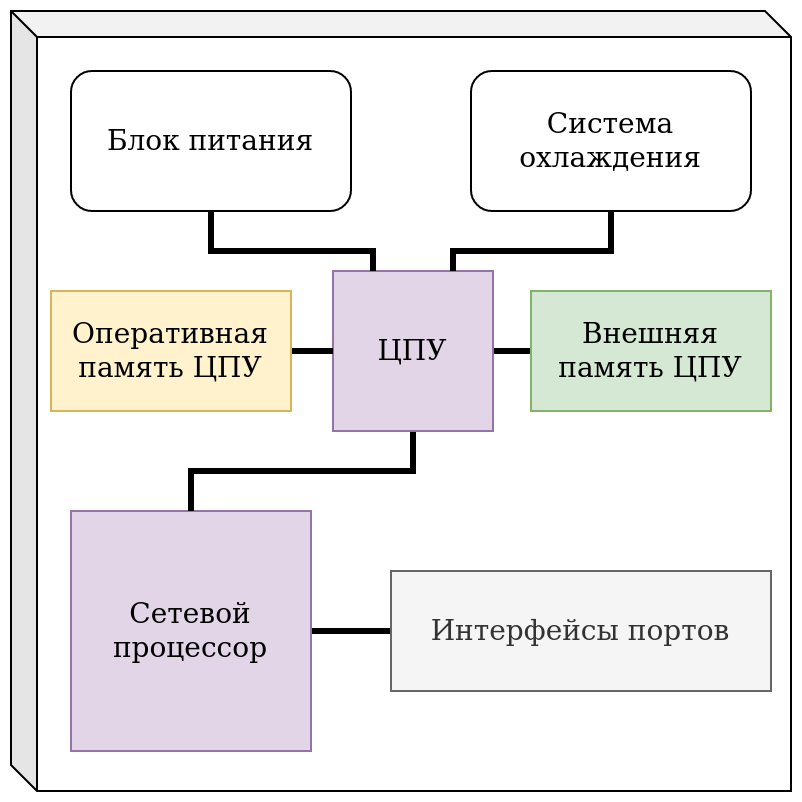
\includegraphics[width=0.5\textwidth]{switch}
            \caption{Структурная схема коммутатора}
            \label{image_switch}
        \end{figure}

        Коммутатор, функционирующий под управлением протокола OpenFlow, 
        включает в себя следующие основные компоненты (рис. \ref{image_switch}):
        
        \begin{itemize}
            \item Сетевой процессор, выполняющий функцию передачи данных. Данное устройство получает пакеты через интерфейсы портов коммутатора, обрабатывает их, исполняя ранее загруженный машинный код, и затем отправляет необходимые пакеты через интерфейсы портов коммутатора.
            \item Центральное процессорное устройство (ЦПУ), выполняющее функцию интерфейса с контроллером ПКС сети, функцию обновления машинного кода сетевого процессора, а также функцию управления питанием и охлаждением коммутатора.
            \item Блоки оперативной и внешней памяти для ЦПУ.
            \item Интерфейсы портов коммутатора.
            \item Блоки питания и система охлаждения.
        \end{itemize}

        Специальное программное обеспечение (СПО) выполняется в среде операционной системы на ЦПУ. 
        СПО включает в себя следующие программные средства: 
        
        \begin{itemize}
            \item агент протокола OpenFlow (коммуникация с контроллером и интерпретация его сообщений);
            \item система трансляции абстракций протокола OpenFlow в язык ассемблера сетевого процессора;
            \item транслятор языка ассемблера сетевого процессора в машинный код;
            \item драйверы сетевого процессора и других устройств коммутатора;
            \item служебное программное обеспечение для управления питанием, охлаждением и пр.
        \end{itemize}

        \subsection{Архитектура сетевого процессора (RuNPU)}
            \label{sect:arch}
            В рамках работы важны лишь некоторые особенности рассматриваемой архитектуры, а именно, отсутствие выделенного ассоциативного устройства памяти и конвейерная архитектура. 
            Данные особенности непосредственно влияют на ограничения, предъявляемые к реализуемым структурам данных.

            В сетевом процессоре используется конвейерная архитектура, каждый конвейер состоит из 10 вычислительных блоков. 
            Вычислительный блок $-$ это набор более низкоуровневых RISC ядер, которые в данной работе не рассматриваются. 
            Каждый вычислительный блок имеет доступ к участку памяти, в котором располагаются микрокод и данные.
            Существует ограничение на количество тактов, которое один пакет может обрабатываться на вычислительном блоке, оно соответствует 25 тактам.
            Данное ограничение обусловлено требованием к производительности сетевого процессора, а именно фиксированное время обработки одного пакета на сетевом процессоре.
            Также один вычислительный блок имеет доступ к 64 килобайтам памяти.
            Из-за особенностей микроархитектуры, отсутствует отдельная область памяти, в которой хранятся данные. Поэтому микрокод содержит в себе все данные,
            необходимые для классификации пакетов.

            \begin{figure}[h]
                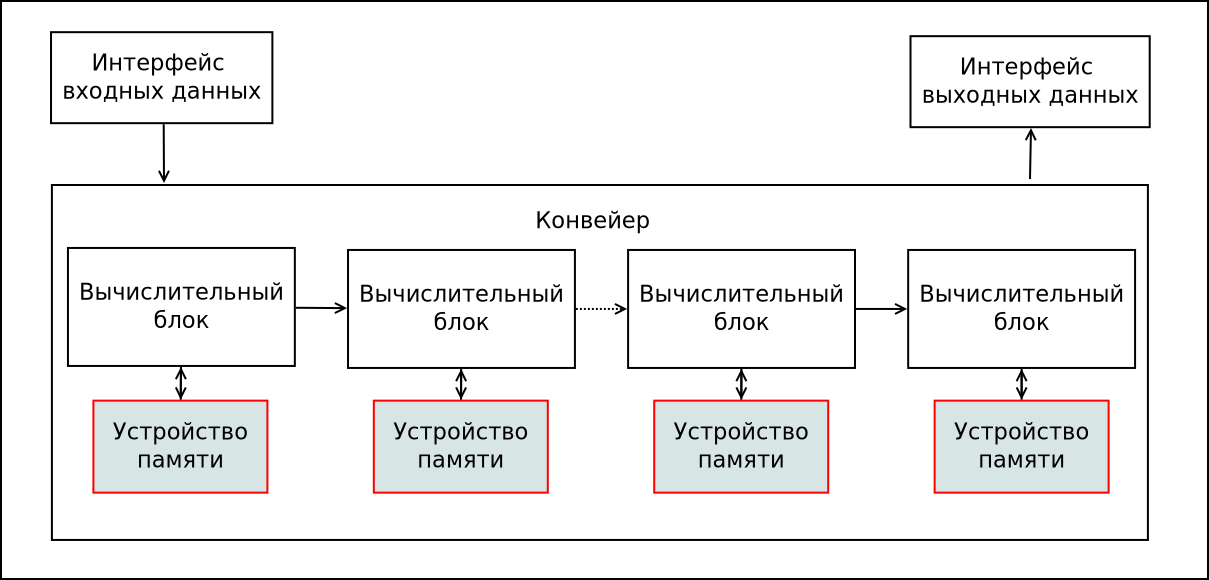
\includegraphics[width=\textwidth]{npu_all.png}
                \caption{Архитектура рассматриваемого сетевого процессора}
            \end{figure}
            
        \subsection{Язык ассемблера сетевого процессора}
            \label{sect:asm}
            Для описания программ обработки сетевых пакетов в рассматриваемой архитектуре сетевого процессора используется язык ассемблера.
            Вычислительный блок конвейера содержит единственный регистр общего назначения длиной 128 бит (регистр-аккумулятор), который выступает в качестве регистра-операнда и/или регистра-результата команды.

            Память, доступ к которой осуществляется через команды, разделена на нескольких частей:
            \begin{itemize}
                \item область заголовка пакета;
                \item область метаданных (размер заголовка, номер порта, на который пришел пакет, маска выходных портов, пользовательские метаданные и др.).
            \end{itemize}

            Также вычислительный блок конвейера содержит регистр смещения. При выполнении команд, 
            осуществляющих доступ в область памяти используется адрес равный сумме адреса, 
            прописанного в команде, и значения регистра смещения.

            Язык ассемблера сетевого процессора предназначен для описания программ, 
            которые исполняются вычислительным блоком конвейера. 
            В рассматриваемом языке присутствуют следующие классы инструкций:
            \begin{itemize}
                \item Инструкции для работы с регистром.
                \item Инструкции арифметических операций.
                \item Инструкции битовых операций.
                \item Инструкции для условного и безусловного перехода на метку.
                \item Инструкция записи в регистр выходного порта.
            \end{itemize}
            Также есть возможность использовать директивы имитационной модели $\#define$ и $\#include$, 
            которые позволяют, например, задавать константы.
           
            Язык ассемблера сетевого процессора также поддерживает специальные команды 
            для вставки деревьев поиска. Директива \texttt{tree\underline{ }in} включает дерево 
            поиска по точному совпадению. В качестве параметра директивы указывается имя файла, 
            строки которого содержат пары \texttt{<значение, метка перехода>}. 
            Директива \texttt{tree\underline{ }lpm} включает дерево поиска по совпадению наибольшего 
            префикса. В качестве параметра директивы указывается имя файла, 
            строки которого содержат тройки \texttt{<начало диапазона, длина префикса, метка перехода>}.

            На программу на языке ассемблера рассматриваемого сетевого процессора накладываются 
            следующие ограничения:
            \begin{itemize}
                \item Максимальная битовая длина сравниваемого значения в командах условного перехода 
                    и файлах деревьев поиска равна 64 битам.
                \item Метки переходов, содержащиеся в командах и файлах деревьев поиска, 
                    должны встречаться в программы после команды или директивы соответственно. 
                    Это требование обусловлено архитектурой вычислительного конвейера сетевого 
                    процессора, в котором не допускается переход к командам, 
                    записанным в памяти по меньшему адресу, чем адрес текущей исполняемой команды.
            \end{itemize}

            Важной особенностью также является отсутствие отдельной области памяти для данных программы. 
            Данные задаются в виде аргументов команд и являются неотделимой частью машинных команд.

    \section{Постановка задачи}
        %В данной главе представлена постановка задачи. 
    \subsection{Неформальная постановка задачи}
    \if 0
        Необходимо исследовать применимость существующих алгоритмов сжатия данных в существующей архитектуре СП (RuNPU).
        Рассматриваемые алгоритмы должны удовлетворять следующим условиям:
        \begin{itemize}
            \item Размер итоговой таблицы потоков не должен превышать 512 Кб.
            \item Потери данных при использования алгоритмов сжатия не должны быть значительными.
            \item Сжатую таблицу потоков должно быть возможно использовать без декомпрессии.
        \end{itemize}
    \fi
    Рассматривается коммутатор, функционирующий под управлением протокола OpenFlow,
    описанного в разделе~\ref{sect:openflow}. Коммутатор работает под управлением сетевого
    процессора (RuNPU), архитектура которого описана в разделе~\ref{sect:arch}.
    Сетевой процессор работает под управлением программы на языке ассемблера, которая получается 
    путём трансляции таблиц потоков OpenFlow

    Пусть имеется таблица потоков OpenFlow, содержащая в себе правила с признаками с 
    точным совпадением и маскирующие признаки. Имеется транслятор таблиц потоков, с помощью которого
    получается программа обработки сетевых пакетов на языке ассемблера. То есть классификацию 
    полученного пакета по этой таблице потоков, то есть нахождение в таблице правила 
    с наибольшим приоритетом, идентифицирующим обрабатываемый пакет. В данный момент
    программа на языке ассемблера при большом количестве правил в таблице потоков может занимать
    объём памяти в несколько раз больший, чем ограничения архитектуры (см. раздел~\ref{sect:arch}).

    Таким образом, возникает задача разработки алгоритмов сжатия таблиц потоков,
    для уменьшения объёма памяти занимаемого программ на языке ассемблера, получаемых из
    таблиц потоков путём их трансляции. При этом программа получаемая из сжатой таблицы потоков 
    должна быть идентична программе получаемой из исходной таблице потоков.



    
    \subsection{Формальная постановка задачи}
        \label{sect:problem}
        Введём формализацию OpenFlow таблиц.
        Упорядоченное множество всех рассматриваемых признаков в правилах обозначим \(I=\{m_1,m_2,\ldots,m_k\}\). 
        Каждый признак \(m_i\) из множества признаков \(I\) характеризуется битовой строкой, некоторой длины \(m_i \in \{0, 1, *\}^W_i\),
        в данном случае символ \(*\) обозначает любой бит. При этом, если \(\exists m_i^j \in m_i\), такое, что 
        \( m_i^j = *\), то для \( \forall m_i^k \), где \(k > j\), то \( m_i^k = *\). Длиной признака обозначим \(len(m_i) = W_i\)

        Представим таблицу потоков в виде множества правил \(R=\{r_1,r_2,\ldots,r_n\}\). С каждым правилом \(r_i\) связаны:
        \begin{itemize}
            \item номер \(i\);
            \item приоритет \(p_i\in Z_+\);
            \item вектор значений признаков \(f_i=\{f_i^1,f_i^2,\ldots,f_i^k\}\), где \(f_i^j\) соответствует значению признака \(m_j\in I\). % и \(f_i^j\in D(m_j)\cup\{*\}\), \(j=\overline{1,k}\).
            \item Набор действий, \(A_i = \{a_1, a_2, \ldots, a_z\} \), которые определяют дальнейшие действия сетевого процессора над пакетом.
        \end{itemize}

        Будем говорить, что заголовок пакета \(x\) и его метаданные с вектором значений признаков \(g=\{g^1,g^2,\ldots,g^k\}\) (далее \(x \rightarrow g\)),
        соответствуют правилу \(r_i\in R\) с вектором значений признаков \(f_i=\{f_i^1,f_i^2,\ldots,f_i^k\}\) 
        и приоритетом \(p_i\) (правило \(r_i\in R\) идентифицирует пакет с вектором значений признаков \(g\)), если:

        \begin{enumerate}
            \item вектор значений признаков \(g\) соответствует вектору значений признаков \(f_i\), 
                то есть \(\forall g_i \in g\), \(len(g_i) = len(f_i)\). И \(\forall f_i^{lj} \in f_i^l\), \(f_i^{lj} \in \{*, g^{lj}\}\), \(l=\overline{1,k}\);
            \item приоритет \(p_i\) максимален среди всех правил \(r_j\in R\), для которых \(g\) соответствует вектору значений признаков \(f_j\).
        \end{enumerate}

        Множество \(R\) также должно удовлетворять следующему ограничению. 
        Для любых двух правил \(r_i,r_j\in R,r_i\not= r_j\), если их вектора значений пересекаются, то есть существует набор значений признаков, 
        который соответствует векторам значений признаков обоих правил, то \(p_i\not= p_j\). 
        Например, правила с векторами значений признаков \(f_i=\{110, 011, 1*\}\) и \(f_j=\{11*, 011, 11\}\) должны иметь разный приоритет, 
        так как набор значений признаков \(g=\{110, 011, 11\}\) соответствует обоим правилам.
        
        Введём функцию идентификации заголовка пакета \(x \rightarrow g\) в таблице потоков \(R\) и обозначим её \(R(x)\).
        Функция идентификации заголовка возвращает набор действий, соответствующий правилу, идентифицирующему заголовок пакета \(x \rightarrow g\).
        Таким образом \(R(x) = A_{r_i}\), где \(A_{r_i}\) набор действий правила \(r_i \in R\).

        Введём понятие аналогичности множеств \(R_1\) и \(R_2\).
        Множество \(R_1\) аналогично множеству \(R_2\), если для любого заголовка пакета, для которого существует идентифицирующее его правило \(r_i \in R_1\), 
        найдётся правило идентифицирующее его в множестве \(r_j \in R_2\), при этом \(A_i = A_j\).

        Необходимо разработать алгоритм сжатия таблиц потоков, который будет переводить исходное множество $-$ \(R_1\), соответствующее исходной таблице потоков, в
        новое множество \(R_2\), которое соответствует новой таблице потоков.
        \begin{enumerate}
            \item Множество \(R_1\) должно быть аналогично множеству \(R_2\).
            \item Мощность множества \(R_2\) должна быть меньше либо равно мощности множества \(R_1\).
        \end{enumerate}

        Введём операцию последнего значащего бита признака \(last(m_i) = j\), такое, что \(m_i^j \in \{0, 1\}\) и \(m_i^{(j+1)} = *\). 
        Назовём правила \(r_i \in R\) и \(r_j \in R\) похожими, 
        если для \(\forall u \in len(f_i)\) верно, что \(last(f_i^u) = last(f_j^u) = l\), при этом \(f_i^{ul} \neq f_j^{ul}\), и \(A_i = A_j\).



    \section{Обзор существующих алгоритмов сжатия}
        \subsection{Цель и задачи обзора}
        Целью данного обзора является выбор алгоритмов сжатия для применения в сетевом процессорном устройстве. 
        Необходимость применения алгоритмов сжатия обусловлена недостатком объёма памяти конвейера сетевого процессорного устройства.
        
        В настоящем обзоре будут использоваться следующие критерии:
        \begin{enumerate}
            \item Отношение объёма памяти занимаемого таблицей классификации после применения алгоритма сжатия, 
                к изначальному объёму памяти занимаемому таблицей классификации (Степень сжатия).
            \item Оценка сложности сжатия.
            \item Возможность использования без декомпрессии таблиц классификации $-$ 
                из-за ограничений рассматриваемого сетевого процессорного устройства сжатые таблицы классификации 
                должны представляться как код ассемблера.
            \item Использование внешней памяти $-$ необходимость использования внешней памяти 
                для использования сжатых таблиц классификации без декомпрессии.
        \end{enumerate}

        Данные критерии обусловлены особенностями рассматриваемой архитектуры СПУ. 
        Критерий \textbf{степень сжатия} необходим для оценки эффективности работы алгоритма сжатия.
        Критерий \textbf{оценки сложности сжатия} необходим для оценки накладных расходов на центральный процессор коммутатора при использовании рассматриваемого
        алгоритма сжатия.
        Критерий \textbf{возможности использования сжатых таблиц потоков без декомпрессии} обусловлен ограничениями архитектуры СПУ, а именно
        отсутствием адресуемой памяти в вычислительных блоках конвейера и ограниченным набором команд доступных СПУ (Раздел ~\ref{sect:asm}).
        Критерий \textbf{необходимости использования внешней памяти} обусловлен дополнительными накладными расходами при обработке сетевым процессорным устройством 
        заголовков сетевых пакетов.

        Для описания алгоритмов сжатия в обзоре будет использована терминология описанная в разделе~\ref{sect:problem}. 

    \subsection{Рассматриваемые алгоритмы сжатия}
        \subsubsection{Распространённые алгоритмы}
            Под распространёнными алгоритмами сжатия будем понимать алгоритмы, 
            которые сжатые данные представляют в бинарном виде~\cite{kodituwakku2010comparison}. 
            Примером таких алгоритмов может служить:
            \begin{itemize}
                \item алгоритм Хаффмана,
                \item JPEG,
                \item LWZ,
                \item zip.
            \end{itemize}
            
            Рассмотрим критерии для данного класса алгоритмов. Различные алгоритмы в данной группе имеют различную \textbf{степень сжатия}, 
            которая колеблется от 0.3 до 0.8. Большинство рассматриваемых алгоритмов имеют квадратичную или кубическую \textbf{сложность сжатия} 
            от объёма сжимаемых данных. Так как сжатые данные после применения алгоритмов из данной группы представляются в бинарном виде,
            \textbf{невозможно использовать сжатые таблицы классификации без декомпрессии}. И некоторые алгоритмы из рассматриваемой группы требуют доступ к \textbf{внешней памяти}.
        \subsubsection{Алгоритм оптимального кеширования}
            Данный алгоритм основан на построение дерева поиска правил относительно их частот~\cite{rottenstreich2016optimal}, при этом, в данное дерево
            попадают только правила с определёнными частотами использования (далее популярность). 
            Правила, не попавшие в основное дерево, хранятся на центральном процессоре коммутатора и  доступ к ним осуществляется по запросу СПУ.
            
            Для описания данного алгоритма потребуется ввести дополнительные обозначения. Введём понятие распределения заголовков пакетов \(P\),
            где \(p_x\) обозначает вероятность получения пакета \(x \rightarrow g=\{g^1,g^2,\ldots,g^k\}\).
            Также введём понятие коэффициента правильности \(T_P(R_1, R_2)\), где \(R_1\) и \(R_2\) две различные таблицы потоков. 
            Таким образом коэффициент правильности обозначает вероятность того, что заголовок пакета, согласно распределению \(P\),
            будет в идентифицироваться правилами \(r_1 \in R_1\) и \(r_2 \in R_2\) и их наборы действий совпадают \(A_1 = A_2, A_1 \in r_1, A_2 \in r_2\).
            
            \[T_P(R_1, R_2) = \sum_{x \rightarrow g, R_1(x) = R_2(x)} p_x\]

            Введём оптимальное значение коэффициента правильности для заданной таблицы потоков \(R\), числа правил \(n\) и распределения заголовков \(P\).
            \[\zeta(n, R, P) = \max_{R_i, |R_i| <= n} T_P(R, R_i)\]
            
            Таким образом алгоритму необходимо найти и построить таблицу потоков \(R_a\), основанную на данной таблице потоков \(R\)
            с наименьшим количеством правил \(n_0\) и максимальные оптимальным коэффициентом правильности \(\zeta(n, R, P)\).
            Пусть \(p^i\) популярность (вероятность) выбора правила \(r_i \in R\), в соответствие с распределением заголовков \(P\). Пусть
            правила в таблице потоков \(R\) расположены в порядке не возрастания их популярности. Тогда:
            \[\zeta(n, R, P) \geq \sum_{i \in [1, n]} p^i + 1 - \sum_{i \in [1, n_0]} p^i \geq n/n_0\]

            Рассмотрим критерии для данного алгоритма: \textbf{Степень сжатия} данного алгоритма зависит от распределения частот использования префиксов, от 0.1 до 0.9.
            Данный алгоритм имеет квадратичную \textbf{сложность построения}. Сжатые таблицы классификации \textbf{возможно использовать без декомпрессии}.
            Для работы данного алгоритма \textbf{требуется внешняя память}, так как часть префиксов, которая не попала в выборку наиболее часто используемых хранится в
            памяти центрального процессора коммутатора.
        \subsubsection{Алгоритм Recursive endpoint cutting}
            Данный алгоритм основан на применении дерева HyperSplit, а сжатие производится за счёт удаления дублирующихся правил.~\cite{chang2019fast}
            Данный алгоритм поддерживает добавление и удаление правил в таблице потоков.

            Под дублирующимися правилами в таблице потоков понимаются следующие правила:
            \begin{itemize}
                \item правило, содержащиеся в вершине дублируется правилом в вершине, являющийся листом для данной вершины (частично дублирующиеся правило);
                \item правило, содержащиеся в вершине дублируется правилами во всех вершинах, являющихся листьями для данной вершины (полностью дублирующиеся правило).
            \end{itemize}
            Соответственно дублирующиеся правила перемещаются наверх дерева, что позволяет удалить полностью дублирующиеся правила.
            
            Данный алгоритм рекурсивно использует NewHypersplitstore для удаления повторяющихся правил из дерева, которое строится в настоящее время. 
            Затем удаленные повторяющиеся правила собираются в виде второй таблицы правил, называемой рекурсивной таблицей, для построения второго дерева. 
            Возможно, что во втором дереве  все еще существуют повторяющиеся правила, и некоторые из них также удаляются и используются для построения третьего дерева. 
            Этот процесс построения дерева выполняется рекурсивно до тех пор, пока в последнем дереве не будет дублированных правил. 

            Рассмотрим критерии для данного алгоритма: \textbf{Степень сжатия} данного алгоритма приблизительно равна 0.15.
            Данный алгоритм имеет \textbf{сложность построения} \(n*log(n)\). Сжатые таблицы классификации \textbf{возможно использовать без декомпрессии}.
            Для работы данного алгоритма \textbf{не требуется внешняя память}, так как всё сжатие происходит в момент трансляции таблицы потоков в
            программу на языке ассемблера.
        \subsubsection{Алгоритм с использованием битовых векторов для представления таблиц потоков}
            Данный алгоритм основан на применение битовых строк для представления таблиц потоков~\cite{shi2020msbv}. А именно таблица потоков разбивается на несколько частей,
            в каждой из которых для всех битов префиксов записывается два значения: подходит ли данный префикс, если в искомой строке 1, 
            подходит ли данный префикс, если в искомой строке 0. Таким образом поиск по таблицам потоков будет состоять из последовательного применения 
            операции and.
            Все совпадающие поля делятся на \(\frac{L}{s}\) sub-полей, где \((1 ≤ s ≤ L)\) обозначает длину подполя в битах. 
            \(K_j (j = 0,1, ..., Ls − 1)\) обозначает бит в подполе j. StrideBV уменьшает количество подходящих поисков, 
            а также уменьшает задержку поиска.             

            Рассмотрим критерии для данного алгоритма: \textbf{Степень сжатия} данного алгоритма равна 0.5.
            Данный алгоритм имеет квадратичную \textbf{сложность построения}. Сжатые таблицы классификации \textbf{возможно использовать без декомпрессии}.
            Для работы данного алгоритма \textbf{требуется внешняя память}.
            %\subsubsection{Укороченное КД-дерево}
        %   Данный алгоритм основан на построение обычного КД-дерева. Разберём простой алгоритм построения КД-дерева:
        %   \begin{itemize}
        %    \end{itemize}
        \subsection{Сравнение алгоритмов сжатия}
             Для сравнения алгоритмов сжатия рассмотрим Таблицу~\ref{tab:tab1}. Сравнение будет проводится по следующим критериям:
        \if 0
        \begin{table}[ht]
            \caption{Сравнение алгоритмов сжатия.}\label{tab:tab1}
            \begin{tabular}{|m{4.3cm}|m{2.5cm}|m{2cm}|m{2cm}|m{3.3cm}|}
                \hline
                \bf Название алгоритма сжатия & \bf Cложность построения & \bf Степень сжатия & \bf Внешняя память & \bf Необходимость декомпрессии \\
                \hline
                Алгоритм оптимального кеширования & $O(N^2)$ & \(0.1 \ldots 0.9\) & да & нет \\
                \hline
                Алгоритм рекурсивного удаления & $O(N*log(N))$ & \(0.1\) & нет & нет \\
                \hline
                Алгоритм с использованием битовых строк & $O(\frac{W}{K}*L)$ & \(0.5\) & нет & нет \\
                \hline
                Распространённые алгоритмы & $O(K*\log_2{N})$ & \(0.1 \ldots 0.8\) & нет & да \\
                \hline
            \end{tabular}
        \end{table}
        \fi
       %\if 0 
        \begin{table*}[!t]
            \centering
            \caption{Сравнение алгоритмов сжатия.}\label{tab:tab1}
            \begin{tabularx}{\textwidth}{m{4.3cm}m{2.5cm}m{2cm}m{2cm}m{3.3cm}}
 %{@{}l*{10}{C}c@{}} %{|m{3.5cm}|m{2.5cm}|m{2cm}|m{3.5cm}|m{4cm}|}
                \toprule
                \bf Название & \bf Cложность построения & \bf Степень сжатия & \bf Внешняя память & \bf Необходимость декомпрессии \\
                \midrule
                Оптимальное кеширование & $O(N^2)$ & \(0.1 \ldots 0.9\) & да & нет \\
                Рекурсивное удаления & $O(N*log(N))$ & \(0.1\) & нет & нет \\
                Использование битовых строк & $O(\frac{W}{K}*L)$ & \(0.5\) & нет & нет \\
                Распространённые алгоритмы & $O(K*\log_2{N})$ & \(0.1 \ldots 0.8\) & нет & да \\
                \bottomrule
            \end{tabularx}
        \end{table*}
        %\fi
        
        У каждого рассмотренного алгоритма сжатия есть свои достоинства и недостатки, рассмотрим их:
        \begin{enumerate}
            \item \textbf{Алгоритм оптимального кеширования} \(-\) имеет наибольший коэффициент сжатия, и быстро реализуем в рассматриваемой архитектуре сетевого процессорного устройства. 
                Необходимость использования внешней памяти накладывает дополнительные расходы на обработку некоторых пакетов.
            \item \textbf{Алгоритм рекурсивного удаления} \(-\) имеет наименьший коэффициент сжатия,
                реализуем сложнее, чем алгоритм оптимального кеширования. При этом данный алгоритм не требует использования внешней памяти.
            \item \textbf{Алгоритм с использованием битовых строк} \(-\) имеет средний коэффициент сжатия, но при этом трудно реализуем в рассматриваемой архитектуре сетевого процессорного устройства.
            \item \textbf{Распространённые алгоритмы сжатия} \(-\) в среднем имеют хорошие коэффициенты сжатия, но при этом требуется декомпрессия данных.
        \end{enumerate}
        
        Таким образом, на основе обзора для дальнейшей реализации были выбраны два алгоритма сжатия данных. Алгоритм оптимального кеширования и алгоритм с использованием битовых строк.

        \subsection{Выводы}
        В данной главе был проведён обзор существующих алгоритмов сжатия, а именно: распространённые алгоритмы сжатия, алгоритм оптимального кеширования, алгоритм рекурсивного удаления 
        и алгоритм с использованием битовых строк.
    \section{Эмулятор сетевого процессора}
        Эмулятор сетевого процессора $-$ программа написанная на языке программирования $python3$, которая позволяет эмулировать работу сетевого процессора, 
        а именно получать пакеты на любой из 24-х портов, обрабатывать пакет, получая информацию о любой стадии обработки, и отправлять пакет на выходные порты.
        Эмулятор сетевого процессора позволяет оценить количество тактов затраченных на обработку пакета, а также объём памяти затраченный на структуру данных.

        Работа эмулятора сетевого процессора состоит из следующих шагов:
        \begin{enumerate}
            \item \textbf{Макрогенерация.} Производится замена констант, объявленных с помощью 
                директив \texttt{define}, на их числовые значения. Происходит генерация 
                деревьев поиска из значений, записанных в файлах деревьев поиска. 
                При этом директивы включения деревьев поиска заменяются на соответствующие наборы 
                команд и меток перехода.
            \item \textbf{Запись программы во внутреннее представление.} Команды полученной на 
                предыдущем шаге программы переводятся во внутреннее представление программы 
                имитационной модели, моделирующее адресное пространство вычислительного конвейера.
            \item \textbf{Обработка входных пакетов.} Происходит последовательная обработка 
                входных пакетов с записью выходных пакетов. Также на этом шаге в режиме отладки 
                возможна запись информации о последовательности выполнения команд.
            \item \textbf{Вывод статистической информации.} По результатам обработки входных 
                пакетов выводится количество обработанных пакетов, среднее число тактов, 
                затраченное на обработку одного пакета, объем занимаемой программой памяти, 
                данные по энергопотреблению и др.
        \end{enumerate}

        \subsection{Описание программных средств эмулятора сетевого процессора}
            Передача пакетов на порты сетевого процессора осуществляется с помощью файлов $.pcap$, в которых можно описать поступление пакетов на каждый порт в определённые моменты времени.
            В данной работе, не уменьшая общности, будет рассматриваться только один порт эмулятора сетевого процессора. Так как для каждого входного
            порта используется соответствующий конвейер. Изначально, в конвейере эмулятора сетевого процессора был реализован один вычислительный блок.
            Для проведения экспериментального исследования в данной работе, необходимо внести изменения в эмулятор сетевого процессора, а именно увеличить количество вычислительных блоков 
            в конвейере до 10.
        \subsection{Программные средства разработанные для проведения экспериментального исследования}
            Для проведения экспериментального исследования в рамках данной работы, необходимо разработать генератор сетевого трафика, который должен удовлетворять следующим требованиям:
            \begin{itemize}
                \item Возможность генерации L2 и L3 трафика.
                \item Возможность использовать наперёд заданную базу префиксов или mac-адресов для генерации трафика.
                \item Возможность использовать для генерации трафика заданное количество случайных префиксов или mac-адресов.
                \item Возможность сохранить базу использованных префиксов или mac-адресов.
                \item Возможность задать распределения времени поступления пакетов.
            \end{itemize}
            Для реализации будет использовать язык программирования $python3$, так как существует открытая библиотека $scapy$, которая позволяет работать с L2 и L3 трафиком,
            а так же позволяет сохранять сгенерированные пакеты в $.pcap$ файлы, что необходимо, для дальнейшего использования в эмуляторе сетевого процессора.
    \section{Система трансляции таблиц потоков в язык ассемблера сетевого процессорного устройства}
        В данной главе приводится описание системы трансляции таблиц потоков OpenFlow~\cite{andrewmonetec}. Также будет представлено описание
        структур данных, использующихся для промежуточного представления таблиц потоков, и разработанных алгоритмов сжатия таблиц потоков и трансляции
        сжатых таблиц потоков в язык ассемблера СПУ.
        \subsection {Структуры данных}
            \subsubsection {Структура данных для представления таблиц потоков в виде дерева}
                В системе трансляции для представлении таблицы потоков с набором правил \(R\) используется дерево с помеченными вершинами и дугами.
                С каждой вершиной дерева, кроме вершин-листьев, связаны следующие значения:
                \begin{itemize}
                    \item признак из множества рассматриваемых признаков;
                    \item подмножество набора правил R.
                \end{itemize}

                Структура данных строится по следующим правилам, где \(v\) $-$ вершина дерева, которой соответствует признак \(m\) и подмножество правил \(S \subset R\):
                \begin{enumerate}
                    \item корню дерева соответствует всё множество правил \(R\);
                    \item если \(M\) $-$ множество всевозможных значений признака \(m\) в правилах из подмножества \(S\), то для каждого значения \(f \in M\)
                        у вершины \(v\) существует потомок, к которому ведёт дуга с пометкой \(f\).
                    \item если вершины \(u\) $-$ потомок вершины \(v\) в которую ведёт дуга с пометкой \(f\), то подмножество правил вершины \(u\) состоит только из
                        правил в \(S\), у которых значение признака \(m\) равно \(f\).
                \end{enumerate}

                Описанная структура данных позволяет выполнять поиск идентифицирующего обрабатываемый пакет правила в таблице потоков.
            \subsubsection{Структура данных для представления таблиц потоков в виде АВЛ дерева}
                В прошлой работе~\cite{nik_avl} была разработана структура данных для представления таблиц классификации в виде АВЛ дерева.
                Аналогично таблицу потоков можно также представить в виде АВЛ дерева, с каждой вершиной АВЛ дерева связаны следующие значения:
                \begin{itemize}
                    \item скалярное значение соответствующее набору признаков \(I = {m_1, m_2, \ldots, m_k}\), вычисляемое по расширенному алгоритму представления префиксов 
                        как скалярных величин.
                    \item подмножество набора правил \(R\), соответствующих данному набору признаков.
                \end{itemize}
            \subsubsection{Структура данных для промежуточного представления таблицы потоков}
                Для применения алгоритмов сжатия необходимо промежуточное представление таблицы потоков.
                А именно в дополнение к существующим структурам данных к каждой вершине необходимо добавить следующие значения:
                \begin{itemize}
                    \item Величина \(P(S)\) соответствующая сумме частот использования каждого правила из подмножества \(S \subset R\). 
                        \(P(S) = \sum_{r_i \in S} P(r_i)\).
                    \item Величина \(P(N)\) соответствующая сумме частот использования потомков данной вершины. \(P(N) = \sum_{f_i \in M} P(N(f_i))\).
                        Если у данной вершины нет потоков, то \(P(N) = P(S)\).
                \end{itemize}
        \subsection{Модуль генерации ассемблерного кода}
            В данной работе в трансляторе таблиц потоков интересен модуль генерации 
            ассемблерного кода. В нём реализован алгоритм трансляции структуры данных в программу 
            на языке ассемблера сетевого процессора. Программа строится на основе одного из 
            представлений таблицы потоков, используя соответствующий ему метод. Выходными данными 
            модуля является набор файлов, включающий в себя основной файл программы с кодом 
            на языке ассемблера и файлы деревьев поиска, встречающихся в директивах основного 
            файла программы.

            В данном модуле выделяются следующие внутренние модули:
            \begin{itemize}
                \item \textit{Генератор ассемблерного кода} предоставляет интерфейс модуля 
                    генерации ассемблерного кода.
                \item \textit{Модуль прямого способа трансляции} реализует алгоритм трансляции 
                    прямым способом посредством обхода вершин дерева, 
                    полученного модулем представления таблицы потоков в виде дерева.
                \item \textit{Модуль способа трансляции с кодированием дуг} реализует алгоритм 
                    трансляции способом с кодированием дуг посредством обхода таблиц, полученных 
                    модулем представления таблицы потоков в виде уровней дерева.
                \item \textit{Генератор команд} содержит общие функции для двух способов трансляции,
                    например, функции для добавления записей в файлы деревьев поиска или функцию, 
                    создающую код на языке ассемблера, для загрузки значения поля заголовка 
                    пакета в регистр аккумулятор.
            \end{itemize}

        \subsection{Алгоритмы сжатия}
           \subsubsection{Использованные обозначения}
                Пусть \(node_1\), \(node_2\)~--- вершины дерева, \(value\)~--- некоторое значение признака. Введем следующие обозначения:
                \begin{itemize}
                    \item \(Tree.root\)~--- корневая вершина дерева \(Tree\).
                    \item \(node_1(value)\)~--- потомок вершины \(node_1\), связанный с ней дугой с пометкой \(value\).
                    \item \(node_1.rules\)~--- множество правил, соответствующее вершине \(node_1\).
                    \item \(node_1.edges\)~--- множество пометок дуг, исходящих из вершины \(node_1\).
                    \item \(copy(node_1, val, node_2)\)~--- процедура, которая добавляет к вершине \(node_1\) потомка с дугой, помеченной \(val\), копируя дерево, которое образует вершина \(node_2\).
                    \item \(remove(node_1, val)\)~--- процедура, которая удаляет из вершины \(node_1\), поддерево с дугой помеченной \(val\). 
                    \item \(equals(node_1, node_2)\)~--- функция, которая возвращает \(true\), если деревья, образованные вершинами \(node_1\) и \(node2\) совпадают, иначе возвращает \(false\). При сравнении учитываются связанные с вершинами множества правил и пометки дуг.
                    \item \(isleaf(node_1)\)~--- функция, которая возвращает \(true\), если \(node_1\)~--- лист дерева, иначе возвращает \(false\).
                \end{itemize}
            \subsubsection{Алгоритм предварительной оптимизации таблицы потоков}
                В данном разделе будет описан алгоритм предварительной оптимизации таблиц потоков. Для начала необходимо ввести
                операцию {\bf Same}, которая на вход получает две вершины дерева и возвращает множество правил, которые были получены путём объединения 
                похожих правил.
\begin{lstlisting}[float=htb]
procedure Same(node_1, node_2):
    rules = {}
    for all rule_1 in node_1.rules do
        for all rule_2 in node_2.rules do
            if same(rule_1, rule_2) then
                rules += {rule_1 union rule_2}
            endif
    return rules
\end{lstlisting}
                Для описания алгоритма предварительной оптимизации таблиц потоков необходимо ввести операцию {\bf Optimise}, которая на вход получает
                корень дерева исходной таблицы потоков, а затем рекурсивно объединяет все похожие правила с помощью процедуры {\bf Same}. 
\begin{lstlisting}[float=htb]
procedure Optimise(node):
    if not isleaf(node) then
        for all val_1 in node.edges do
            for all val_2 in node.edges do
                if val_1 not equal val_2 then
                    node.rules += Same(node(val_1), node(val_2))
                endif
        for all val in node.edges do
            Optimise(node(val))
\end{lstlisting}
                После применения процедуры {\bf Optimise} необходимо удалить все листовые вершины, для этого опишем процедуру {\bf Remove}, которая 
                на вход получает корень дерева, а затем рекурсивно удаляет все листовые вершины в которых не осталось правил.
\begin{lstlisting}[float=htb]
procedure Remove(node):
    if not isleaf(node) then
        for all val in node.edges do
            if isleaf(node(val)) and node(val).rules equal {} then
                remove(node, val)
            else
                Remove(node(val))
            endif
\end{lstlisting}
                Тогда полный алгоритм предварительной оптимизации можно описать последовательным применением процедур {\bf Optimize} и {\bf Remove}.

            \subsubsection{Алгоритм оптимального кеширования}
                В этом разделе представлен адаптированный алгоритм оптимального кеширования. 
                Основной его частью является операция разделения исходной таблицы потоков на две. 
                Для применения дальнейшего алгоритма необходимо построить изначальное дерево с дополнительными полями в узлах.
                \begin{itemize}
                    \item Получить набор вершин дерева.
                    \item Отсортировать этот набор в невозрастающем порядке сумм вероятностей вершин.
                    \item Создать второй набор вершин, из которого в последствии будет строится дерево.
                    \item Создать счетчик, хранящий сумму вероятностей вершин во втором наборе вершин.
                    \item Получить первую вершину с максимальной суммой вероятностей.
                    \item Увеличить счетчик на его вероятность.
                    \item Добавить эту вершину во второй набор вершин и удалить из первого.
                    \item Повторять последние три операции, пока счетчик меньше 0.95.
                    \item Построить дерево из второго набора вершин.
                \end{itemize}
                После выполнения этих операций мы получаем два набора вершин, первый из которых отвечает за второстепенное дерево, а второй за первостепенное.
                Первостепенное дерево преобразуется в программу на языке ассемблера, которая загружается в СПУ.

                Подробнее опишем алгоритмы, необходимые для реализации алгоритма оптимального кеширования.
                Для начала опишем процедуру {\bf GetList}, которая на вход получает корневую вершину дерева \(Tree.root\). 
                На выходе мы получаем список вершин в которых есть правила.
\begin{lstlisting}
procedure GetList(node):
    nodes = {}
    if node.rules not equal {} then
        nodes += node
    endif
    for all val in node.edges do
        nodes += GetList(node(val))

    return nodes
\end{lstlisting}
                    Также необходима процедура выбора первостепенных вершин {\bf GetBest}, которая на вход получает отсортированный список вершин,
                    и возвращает список первостепенных вершин.
\begin{lstlisting}
procedure GetBest(nodes):
    counter = 0.0
    best_nodes = {}
    for all node in nodes do
        if counter is greater 0.95 then
            break
        endif
        counter += node.prob
        best_nodes += node
    return best_nodes
\end{lstlisting}
    \section{Экспериментальное исследование реализованных алгоритмов сжатия}
        При проведении экспериментального исследования ставились следующие цели:
        \begin{itemize}
            \item Оценка степени сжатия программы на языке ассемблера сетевого процессорного устройства, на различных данных.
            \item Оценка времени обновления таблиц потоков при использовании алгоритмов сжатия, на различных данных.
        \end{itemize}
        \subsection{Методика экспериментального исследования}
            Для оценки параметров необходимо исследовать программу на языке ассемблера, получаемую при использовании
            системы трансляции с алгоритмами сжатия и без. Для каждой программы, с помощью эмулятора сетевого процессорного устройства,
            будут исследоваться следующие параметры:
            \begin{itemize}
                \item Объём памяти занимаемой программой при обработке пакетов на эмуляторе сетевого процессорного устройства.
                \item Среднее время обработки пакета в тактах сетевого процессорного устройства.
            \end{itemize}
            
            Для проведения экспериментального исследования, необходимо последовательно выполнять следующие действия для каждого набора входных данных:
            \begin{enumerate}
                \item Выбрать таблицу потоков для данного эксперимента.
                \item Провести трансляцию выбранной таблицы потоков в программу на языке ассемблера:
                    \subitem $-$ без использования алгоритмов сжатия, обычное дерево;
                    \subitem $-$ без использования алгоритмов сжатия, с АВЛ деревом;
                    \subitem $-$ с использованием разработанных алгоритмов сжатия.
                \item Провести эмуляцию работы сетевого процессорного устройства с полученными программами на языке ассемблера.
                \item Провести оценку результатов полученных в данном эксперименте.
            \end{enumerate}
            \subsubsection{Данные экспериментального исследования}
                Для проведения экспериментального исследования мы будем использовать несколько вариантов таблиц потоков~\cite{braun2014wildcard}. 
                В этом разделе представлены шаблоны таблиц потоков, которые будут использованы для экспериментального исследования.
                \begin{itemize}
                    \item Первый шаблон~--- шаблон правила таблицы потока содержит значения трех атрибутов: номер входного порта, MAC-адрес назначения и MAC-адрес источника.
                    \item Второй шаблон~--- схема правила таблицы потока содержит значения двух атрибутов: Адрес назначения IPv4 и адрес источника IPv4.
                    \item Третий шаблон~--- таблица правил содержит пять атрибутов: номер входного порта, MAC-адрес назначения, ID VLAN, ID заголовка L3-уровня (EtherType) и IPv4-адрес назначения.
                \end{itemize}
                Ниже представлен пример входной таблицы данных:
\lstset{numbers=none}
\begin{lstlisting}
{SRC_MAC , DST_MAC , INSTR}
{SRC_MAC , DST_MAC , INSTR}
+---+-----------+-----------+--------------+
| 1 | :12       | :10:1     | goto_table 1 |
+---+-----------+-----------+--------------+
| 1 | :23:45    | :20       | goto_table 1 |
+---+-----------+-----------+--------------+
| 1 | :0        | :1        | goto_table 1 |
+---+-----------+-----------+--------------+
\end{lstlisting}
\lstset{numbers=left}
                
        \subsection{Результаты экспериментального исследования}
        \begin{figure}[!htbp]
                \centering
            \begin{tikzpicture}
            \begin{axis}[
                width=0.8\textwidth,
                height=0.6\textwidth,
                ylabel={Объём памяти [Кбайт]},
                xlabel={Количество правил},
                y label style={at={(-0.05, 0.5)}},
                ymin=0, ymax=1700,
                xmin=0, xmax=6500,
                %xmode=log,
                %log basis x={2},
                xtick={1000, 2000, 3000, 4000, 5000, 6000},
                ytick={0, 200, 400, 600, 800, 1000, 1200, 1400, 1600},
                legend pos=north west,
                ymajorgrids=true,
                grid style=dashed,
                cycle list name=color list] 
                \addplot+[mark=square] coordinates{(1000, 123.58)(2000, 303.58)(4000, 500.58)(6000, 904.71)};
                \addplot+[mark=square] coordinates{(1000, 312.58)(2000, 546.58)(4000, 1093.58)(6000, 1406.25)};
                \addplot+[mark=square] coordinates{(1000, 125.58)(2000, 246.58)(4000, 382.58)(6000, 421.71)};
                \addplot+[mark=square, color=green] coordinates{(1000, 156.58)(2000, 273.58)(4000, 492.58)(6000, 773.71)};
                \addplot+[mark=none, color=black] coordinates{(0, 512)(7000, 512)};
                \legend{АВЛ дерево, Без сжатия, Алгоритм ОК, Алгоритм REC, Ограничение}
     
            \end{axis}
            \end{tikzpicture}
                \captionsetup{justification=centering}
                \caption{Зависимость затраченного объёма памяти от количества правил в таблице классификации.}
                \label{graph:compmem}
        \end{figure}
        \(p \in {\eta_{N_k^{t^*}}}\) 
        \begin{figure}[!htbp]
                \centering
            \begin{tikzpicture}
            \begin{axis}[
                width=0.8\textwidth,
                height=0.6\textwidth,
                ylabel={Среднее количество тактов},
                xlabel={Количество правил},
                y label style={at={(-0.05, 0.5)}},
                ymin=0, ymax=90,
                xmin=0, xmax=6500,
                %xmode=log,
                %log basis x={2},
                xtick={1000, 2000, 3000, 4000, 5000, 6000},
                ytick={0, 10, 20, 30, 40, 50, 60, 70, 80},
                legend pos=north west,
                ymajorgrids=true,
                grid style=dashed,
                cycle list name=color list] 
                \addplot+[mark=square] coordinates{(1000, 24)(2000, 26)(4000, 27)(6000, 28)};
                \addplot+[mark=square] coordinates{(1000, 32)(2000, 34)(4000, 36)(6000, 38)};
                \addplot+[mark=square] coordinates{(1000, 50)(2000, 54)(4000, 58)(6000, 80)};
                \addplot+[mark=square, color=green] coordinates{(1000, 26)(2000, 28)(4000, 30)(6000, 31)};
                \legend{АВЛ дерево, Без сжатия, Алгоритм ОК, Алгоритм REC}
     
            \end{axis}
            \end{tikzpicture}
                \captionsetup{justification=centering}
                \caption{Зависимость затраченного объёма памяти от количества правил в таблице классификации.}
                \label{graph:compmem}
            \end{figure}

        \subsection{Выводы}
    \section{Заключение}
    В рамках выпускной квалификационной работы разработаны алгоритмы сжатия 
    таблиц потоков OpenFlow.
    Алгоритмы сжатия данных встраиваются в систему трансляции таблиц потоков
    в язык ассемблера сетевого процессора с использованием промежуточных структуры данных. 
    В ходе работы были достигнуты следующие результаты:
    \begin{itemize}
        \item Проведён обзор существующих алгоритмов сжатия данных, в результате обзора были выбраны для реализации алгоритм оптимального кеширования и алгоритм рекуррентного отсечения;
        \item Выбранные алгоритмы сжатия были адаптированная для внедрения в транслятор таблиц потоков;
        \item Разработана программная реализация алгоритмов сжатия данных в трансляторе таблиц потоков;
        \item Проведено экспериментальное исследование разработанных алгоритмов сжатия, использования которых позволило снизить объём памяти, затрачиваемой на хранение таблиц потоков;
        \item Статья по результатам работы подана статья на конференцию SYRCoSE 2021;
    \end{itemize}

    Экспериментальное исследование показало, что применения алгоритмов сжатия позволяет сократить объём используемой памяти в несколько раз.

        В качестве возможных направлений дальнейших исследований можно указать изучение 
        возможности применения более продвинутых алгоритмов сжатия с использованием специализированной TCAM памяти.
\printbibliography{}
\addcontentsline{toc}{section}{\protect\numberline{}Список Литературы}%

\end{document} 
